\documentclass[9pt,a4paper]{extarticle}

\usepackage[utf8]{inputenc}
\usepackage[T1]{fontenc}
\usepackage[spanish,es-nodecimaldot]{babel}
\usepackage{lmodern}
\usepackage{microtype}
\usepackage{geometry}
\usepackage{graphicx}
\usepackage{booktabs}
\usepackage{tabularx}
\usepackage{array}
\usepackage{amsmath,amssymb}
\usepackage{xcolor}
\usepackage{enumitem}
\usepackage{fancyhdr}
\usepackage{hyperref}
\usepackage{caption}
\usepackage{subcaption}
\usepackage{titlesec}
\usepackage{float}
\usepackage{multicol}

\graphicspath{{../img/}}
\geometry{left=15mm,right=15mm,top=16mm,bottom=15mm}
\setlength{\parindent}{0pt}
\setlength{\parskip}{3pt}
\setlist{nosep,leftmargin=4mm}
\captionsetup{font=footnotesize,labelfont=bf,skip=2pt}
\AtBeginEnvironment{thebibliography}{\tiny\setlength{\itemsep}{-1pt}\setlength{\parskip}{0pt}}

\definecolor{navy}{HTML}{102A43}
\definecolor{blue}{HTML}{167D9A}
\definecolor{pale}{HTML}{EAF5F6}
\definecolor{muted}{HTML}{627D98}
\hypersetup{colorlinks=true,linkcolor=blue,citecolor=blue,urlcolor=blue,
  pdftitle={Clasificación de potabilidad del agua con SVM y kernels cuánticos}}
\titleformat{\section}{\color{navy}\bfseries\large}{\thesection.}{0.45em}{}
\titleformat{\subsection}{\color{blue}\bfseries\normalsize}{\thesubsection}{0.45em}{}
\titlespacing*{\section}{0pt}{6pt}{2pt}
\titlespacing*{\subsection}{0pt}{4pt}{1pt}

\pagestyle{fancy}
\fancyhf{}
\fancyhead[L]{\color{navy}\bfseries\footnotesize QUANTATHON CR 2026 / CHALLENGE 2}
\fancyhead[R]{\color{muted}\footnotesize INFORME TÉCNICO}
\fancyfoot[L]{\color{muted}\scriptsize SVM clásica y kernels cuánticos para potabilidad del agua}
\fancyfoot[R]{\color{muted}\scriptsize\thepage}
\renewcommand{\headrulewidth}{0.8pt}
\renewcommand{\headrule}{\hbox to\headwidth{\color{blue}\leaders\hrule height \headrulewidth\hfill}}
\renewcommand{\footrulewidth}{0.3pt}
\setlength{\headheight}{12pt}

\newcommand{\callout}[1]{\begin{center}\colorbox{pale}{\parbox{0.94\linewidth}{\centering\color{navy}\textbf{#1}}}\end{center}}
\newcolumntype{Y}{>{\raggedright\arraybackslash}X}
\newcolumntype{C}{>{\centering\arraybackslash}X}

\begin{document}

{\color{blue}\bfseries\small INFORME TÉCNICO / DOCUMENTACIÓN DEL REPOSITORIO}\par
\vspace{2mm}
{\color{navy}\bfseries\fontsize{21}{23}\selectfont Clasificación de potabilidad del agua con SVM clásica y kernels cuánticos}\par
\vspace{2mm}
{\color{muted}\large Expresividad, desempeño y ruido de ejecución}\par
\vspace{3mm}

\callout{La evidencia cuántica debe leerse como exploratoria: los mejores resultados son casos aislados y todavía no constituyen ventaja sobre una línea base clásica evaluada bajo el mismo protocolo.}

\section*{Resumen ejecutivo}
El repositorio aborda el Challenge 2 de Quantathon CR 2026: clasificar la potabilidad de 3,276 muestras de agua a partir de nueve variables fisicoquímicas. Los mapas Z, ZZ, Pauli y EfficientSU2 se seleccionaron a partir del curso de aprendizaje automático cuántico de IBM \cite{ibm}; el quinto es un mapa propio inspirado en Bhardwaj \cite{custom_fm}. La matriz de kernel se obtiene con el traslape entre estados y se entrega a \texttt{SVC(kernel='precomputed')}.

El análisis actualizado distingue dos preguntas. La primera identifica la configuración de \textbf{mayor expresividad por cada tipo de mapa}, medida en el repositorio como el promedio de todos los valores de la matriz de kernel, incluida la diagonal. La segunda identifica el \textbf{mejor accuracy observado por tipo}. El mapa propio logra el mayor resultado aislado: accuracy 0.917, exactitud balanceada 0.900 y $F_1=0.889$ con $(N,d)=(48,4)$. Sin embargo, su expresividad es 0.161 y su validación cruzada balanceada es 0.555; por ello no se interpreta como evidencia concluyente.

La SVM-RBF clásica, evaluada con tres semillas, obtiene accuracy $0.6123\pm0.0035$, balanced accuracy $0.6061\pm0.0082$ y $F_1=0.5373\pm0.0197$. EfficientSU2 reúne la mayor expresividad (0.575) y un $F_1$ de 0.609, combinación que lo convierte en el candidato más prometedor para ampliar el estudio, aunque su exactitud balanceada actual sea 0.500. Además, la comparación entre kernel ideal y H2 muestra error absoluto estructurado, con MAE 0.185 en entrenamiento y 0.202 en prueba.

\section{Problema y datos}
La etiqueta \texttt{Potability} vale 0 para agua no potable y 1 para potable. El dataset contiene 1,998 muestras de clase 0 y 1,278 de clase 1; hay faltantes en pH (491), sulfato (781) y trihalometanos (162). El caso se relaciona con el ODS 6, aunque un clasificador no sustituye un análisis certificado ni una decisión sanitaria.

En el flujo \textbf{clásico} se imputaron los valores faltantes con la mediana, se estandarizaron las variables y se aplicó SMOTE únicamente dentro del entrenamiento. En el flujo \textbf{cuántico}, debido al reducido número de datos usado en cada experimento, se conservaron solamente filas originales completas para evitar introducir valores imputados o muestras sintéticas. Después se estandarizaron esas observaciones y se aplicó PCA según la dimensión del circuito. En consecuencia, la QSVM utiliza pocos datos observados, con subconjuntos de 16 a 72 muestras de entrenamiento.

La comparación solicitada por el reto enfrenta una SVM clásica y una QSVM basada en
\begin{equation}
K_Q(\mathbf{x}_i,\mathbf{x}_j)
=\left|\langle\phi(\mathbf{x}_i)\mid\phi(\mathbf{x}_j)\rangle\right|^2.
\end{equation}
\par\smallskip\noindent Este informe utiliza únicamente información y figuras generadas dentro del repositorio.

\clearpage
\section{Línea base SVM-RBF clásica}
La línea base usa una división 80/20 estratificada. Dentro de un pipeline se aplica imputación por mediana, \texttt{StandardScaler}, SMOTE y \texttt{SVC(kernel='rbf')}. La búsqueda evalúa $C\in\{0.1,1,10\}$ y $\gamma\in\{\mathrm{scale},\mathrm{auto},0.01\}$ con cinco folds estratificados, seleccionando la combinación por $F_1$. El proceso completo se repite con semillas 42, 123 y 2026.

\begin{table}[H]
\centering\footnotesize
\caption{Resultados clásicos por semilla.}
\begin{tabular}{rcccccc}
\toprule
\textbf{Semilla} & \textbf{Accuracy} & \textbf{Bal. acc.} & \textbf{$F_1$} & \textbf{CV bal. acc.} & \textbf{$C$} & \boldmath$\gamma$\\
\midrule
42   & 0.6143 & 0.5987 & 0.5163 & 0.6377 & 1 & auto\\
123  & 0.6082 & 0.6049 & 0.5403 & 0.6359 & 1 & auto\\
2026 & 0.6143 & 0.6148 & 0.5554 & 0.6237 & 1 & scale\\
\midrule
\textbf{Media} & \textbf{0.6123} & \textbf{0.6061} & \textbf{0.5373} & \textbf{0.6324} & -- & --\\
\textbf{DE} & \textbf{0.0035} & \textbf{0.0082} & \textbf{0.0197} & \textbf{0.0076} & -- & --\\
\bottomrule
\end{tabular}
\end{table}

\begin{figure}[H]
\centering
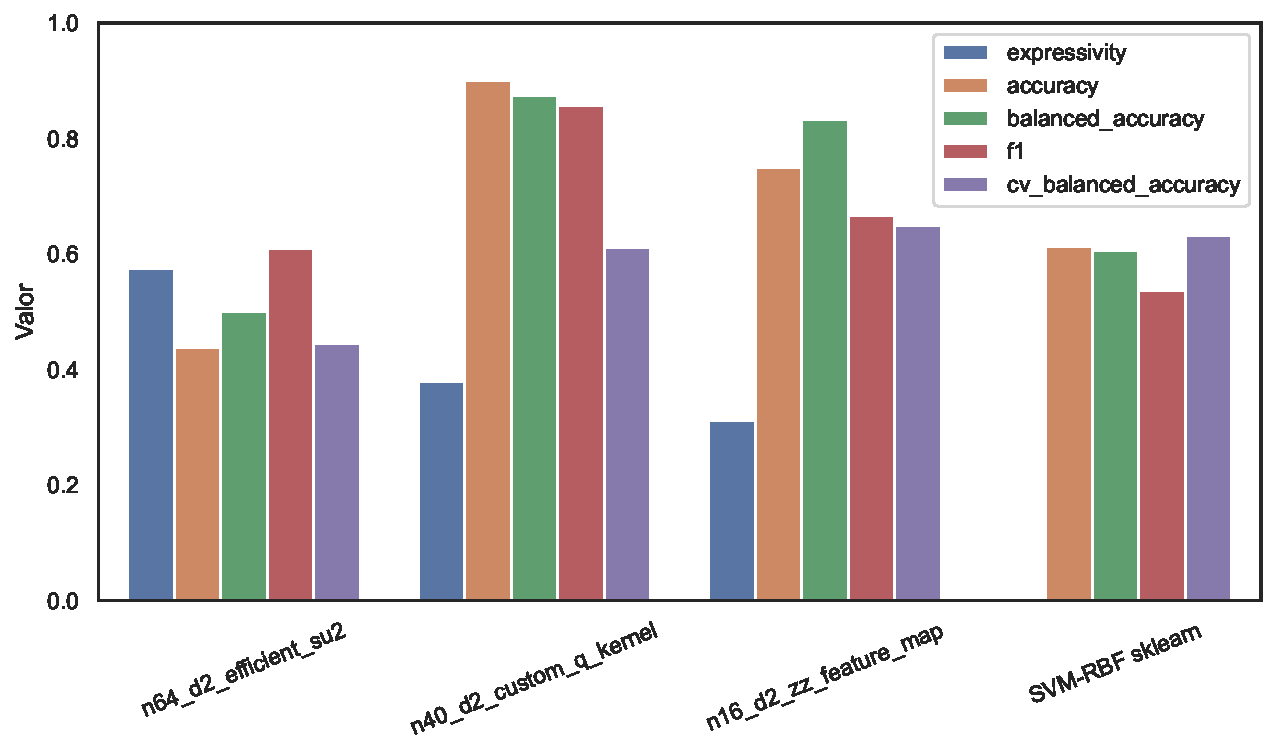
\includegraphics[width=.92\textwidth]{grupo_mayor_expresividad_metricas_vs_sklearn.pdf}
\caption{Métricas generadas para las configuraciones cuánticas más expresivas y la referencia SVM-RBF de sklearn.}
\end{figure}

\section{Criterio de comparación}
La SVM clásica aprovecha las 3,276 filas mediante imputación y balance sintético; la QSVM usa únicamente observaciones completas y subconjuntos pequeños para mantener viable el costo del kernel. Esta diferencia responde a restricciones experimentales, pero impide interpretar las métricas como una comparación pareada. Para una prueba concluyente, ambos métodos deben evaluarse sobre los mismos índices, folds y semillas.

\clearpage
\section{Implementación del kernel cuántico}
\subsection{Los cinco mapas utilizados}
Los cuatro mapas estándar se tomaron como referencia del curso de aprendizaje automático cuántico de IBM \cite{ibm}. Sobre esa base se incorporó un quinto mapa propio:
\begin{enumerate}
  \item \textbf{ZFeatureMap:} codificación mediante rotaciones de fase Z.
  \item \textbf{ZZFeatureMap:} añade interacciones ZZ entre variables.
  \item \textbf{PauliFeatureMap:} usa los términos Pauli Y y ZZ.
  \item \textbf{EfficientSU2:} alterna rotaciones parametrizadas; la configuración expresiva guardada emplea un qubit.
  \item \textbf{Mapa propio:} aplica H, RY, una compuerta T en el segundo qubit y entrelazamiento CZ. Su diseño se basa en la implementación descrita por Bhardwaj \cite{custom_fm}.
\end{enumerate}

\par\smallskip\noindent El cálculo usa \texttt{unitary\_overlap} para estimar
\begin{equation}
K_{ij}=\left|\langle 0|U_{\phi}(\mathbf{x}_j)^{\dagger}
U_{\phi}(\mathbf{x}_i)|0\rangle\right|^2.
\end{equation}
\par\smallskip\noindent Se realizó una optimización basada en la geometría de la matriz: como el kernel de entrenamiento es simétrico, $K_{ij}=K_{ji}$, se calcula únicamente el triángulo superior, se refleja sobre la diagonal y se fija $K_{ii}=1$. Así, el número de evaluaciones pasa de $N^2$ a $N(N-1)/2$, casi la mitad para valores grandes de $N$. El modelo final es \texttt{SVC} con un kernel precomputado.

\begin{figure}[H]
\centering
\begin{subfigure}[t]{.32\textwidth}
\centering
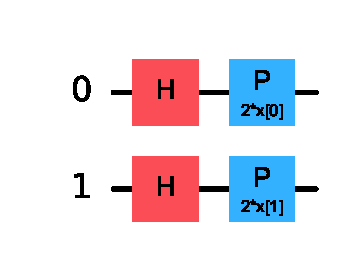
\includegraphics[width=\linewidth,height=2.5cm,keepaspectratio]{n_72_dim_2_z_feature_map_circuito.pdf}
\caption{Z, $(72,2)$.}
\end{subfigure}\hfill
\begin{subfigure}[t]{.32\textwidth}
\centering
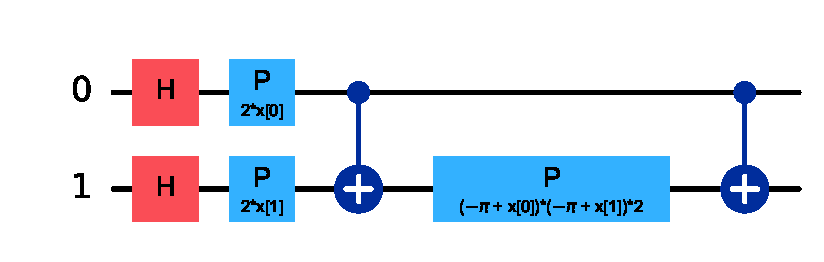
\includegraphics[width=\linewidth,height=2.5cm,keepaspectratio]{n_16_dim_2_zz_feature_map_circuito.pdf}
\caption{ZZ, $(16,2)$.}
\end{subfigure}\hfill
\begin{subfigure}[t]{.32\textwidth}
\centering
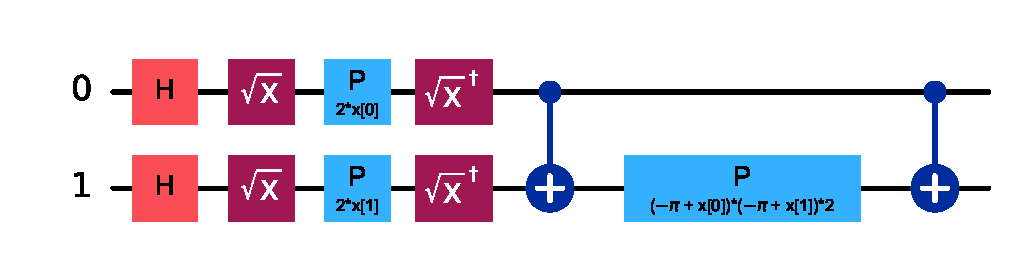
\includegraphics[width=\linewidth,height=2.5cm,keepaspectratio]{n_24_dim_2_pauli_feature_map_circuito.pdf}
\caption{Pauli Y/ZZ, $(24,2)$.}
\end{subfigure}

\vspace{2mm}
\begin{subfigure}[t]{.47\textwidth}
\centering
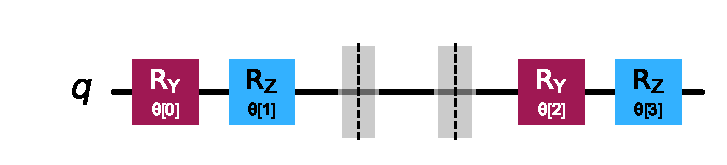
\includegraphics[width=\linewidth,height=2.5cm,keepaspectratio]{n_64_dim_2_efficient_su2_circuito.pdf}
\caption{EfficientSU2, $(64,2)$.}
\end{subfigure}\hfill
\begin{subfigure}[t]{.47\textwidth}
\centering
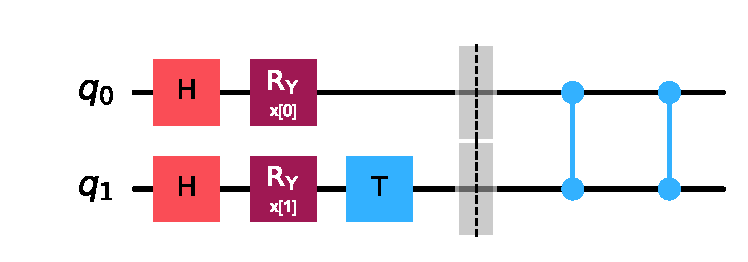
\includegraphics[width=\linewidth,height=2.5cm,keepaspectratio]{n_40_dim_2_custom_q_kernel_circuito.pdf}
\caption{Mapa propio, $(40,2)$.}
\end{subfigure}
\caption{Cinco circuitos generados para las configuraciones de mayor expresividad, uno por tipo de mapa.}
\label{fig:five-circuits}
\end{figure}

\subsection{Costo}
La simetría reduce el entrenamiento de $N^2$ a $N(N-1)/2$ circuitos, pero el crecimiento sigue siendo cuadrático; el test requiere $N_{\rm test}N$. Las cinco configuraciones expresivas tienen profundidades entre 4 y 10 y entre 0 y 2 compuertas de dos qubits.

\subsection{Validación cruzada cuántica}
La validación se calcula únicamente sobre la matriz de kernel de entrenamiento. Se usa \texttt{StratifiedKFold} con cinco folds, mezcla activada y semilla 42. En cada fold se ajusta una nueva \texttt{SVC} precomputada con
\[
K_{\rm train}=K[I_{\rm train},I_{\rm train}],
\]
y se predice la validación con la matriz rectangular
\[
K_{\rm val}=K[I_{\rm val},I_{\rm train}].
\]
\par\smallskip\noindent Para cada fold se calcula balanced accuracy. El valor reportado es la media de los cinco scores y la barra de error es su desviación estándar poblacional. El procedimiento evita que la SVC vea etiquetas de validación, pero no sustituye repetir externamente toda la preparación y generación del kernel.

\subsection{Ventajas del método propuesto}
\begin{itemize}
  \item \textbf{Alta reproducibilidad:} semillas, preparación, familias de mapas, dimensiones, transpilación y métricas se controlan desde una misma configuración; las figuras y tablas se regeneran automáticamente.
  \item \textbf{Modularidad:} el mapa cuántico, el backend, el número de qubits, PCA y la SVC precomputada pueden sustituirse de forma independiente sin rediseñar el flujo completo.
  \item \textbf{Escalado operativo:} la simetría evita evaluaciones duplicadas, los circuitos pueden ejecutarse por lotes y las matrices pueden persistirse para reutilizarse. Esto facilita aumentar muestras y comparar backends, aunque la construcción completa conserva complejidad $O(N^2)$.
\end{itemize}

\clearpage
\section{Cinco configuraciones de mayor expresividad}
La Figura~\ref{fig:expressive-heatmaps} presenta exactamente una configuración por cada tipo de mapa. Todos los mapas de calor comparten escala $[0,1]$, lo que permite comparar directamente la densidad de similitud. EfficientSU2 concentra los valores más altos; Z produce una matriz más dispersa; los mapas propio, ZZ y Pauli ocupan estados intermedios.

\begin{figure}[H]
\centering
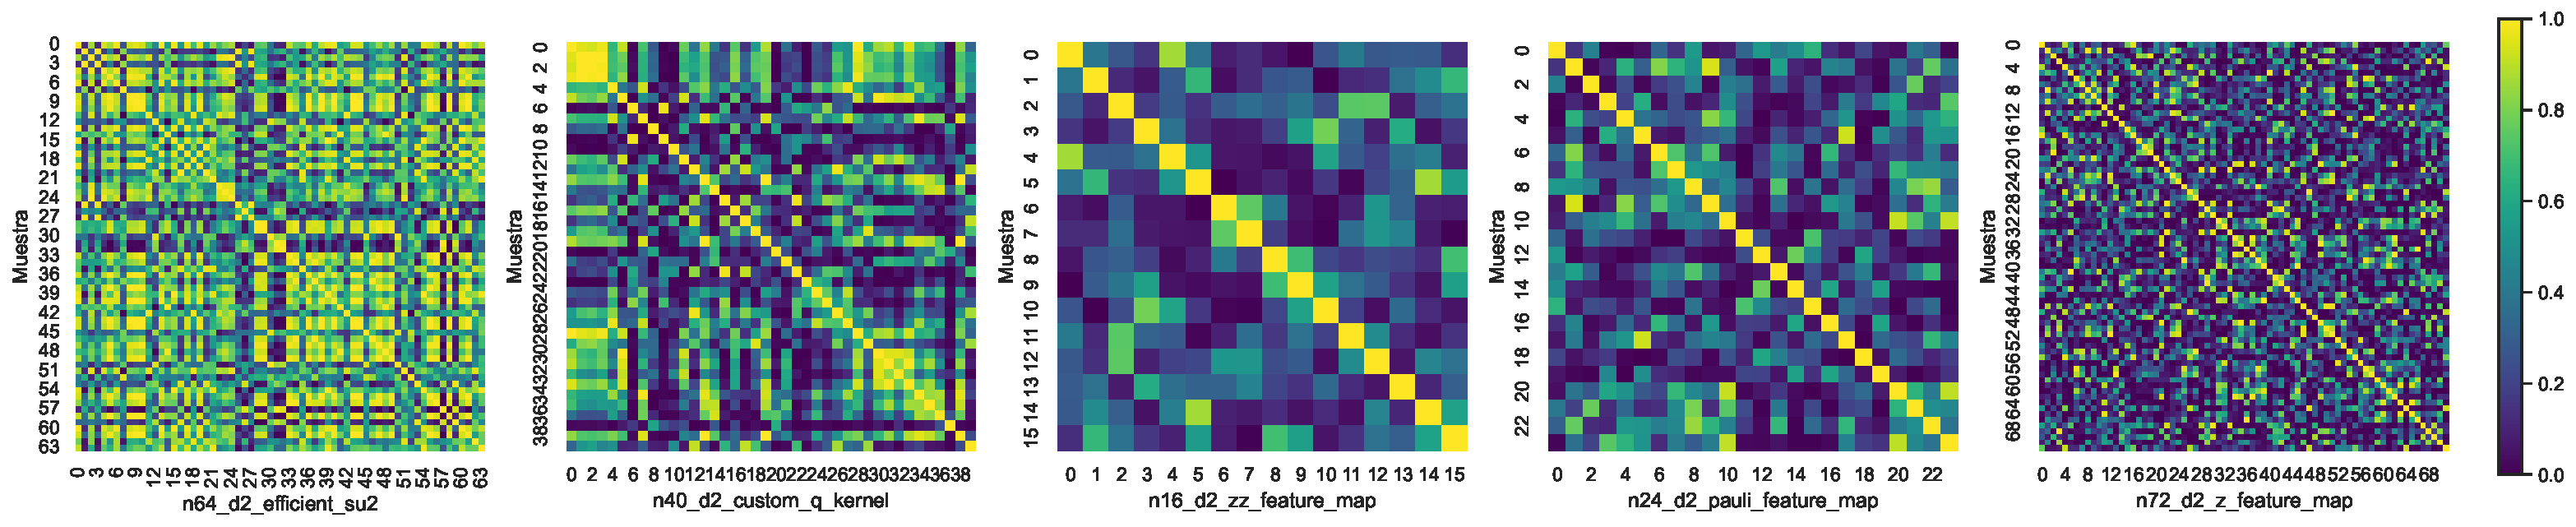
\includegraphics[width=\textwidth]{grupo_mayor_expresividad_heatmaps_escala_0_1.pdf}
\caption{Kernels de entrenamiento de máxima expresividad por tipo: EfficientSU2, propio, ZZ, Pauli y Z.}
\label{fig:expressive-heatmaps}
\end{figure}

\begin{table}[H]
\centering\tiny
\caption{Métricas almacenadas para las cinco configuraciones más expresivas. Las métricas de clasificación se calculan con \texttt{sklearn}.}
\label{tab:expressive}
\begin{tabular}{rrlccccc}
\toprule
$N$ & $d$ & \textbf{Mapa} & \textbf{Expr.} & \textbf{Acc.} & \textbf{Bal. acc.} & \textbf{$F_1$} & \textbf{CV bal. $\pm$ DE}\\
\midrule
64 & 2 & EfficientSU2 & 0.575 & 0.438 & 0.500 & 0.609 & $0.445\pm0.051$\\
40 & 2 & Propio & 0.380 & 0.900 & 0.875 & 0.857 & $0.612\pm0.101$\\
16 & 2 & ZZ & 0.311 & 0.750 & 0.833 & 0.667 & $0.650\pm0.200$\\
24 & 2 & Pauli Y/ZZ & 0.293 & 0.500 & 0.625 & 0.400 & $0.433\pm0.097$\\
72 & 2 & Z & 0.255 & 0.389 & 0.375 & 0.267 & $0.434\pm0.021$\\
\bottomrule
\end{tabular}
\end{table}

\begin{figure}[H]
\centering
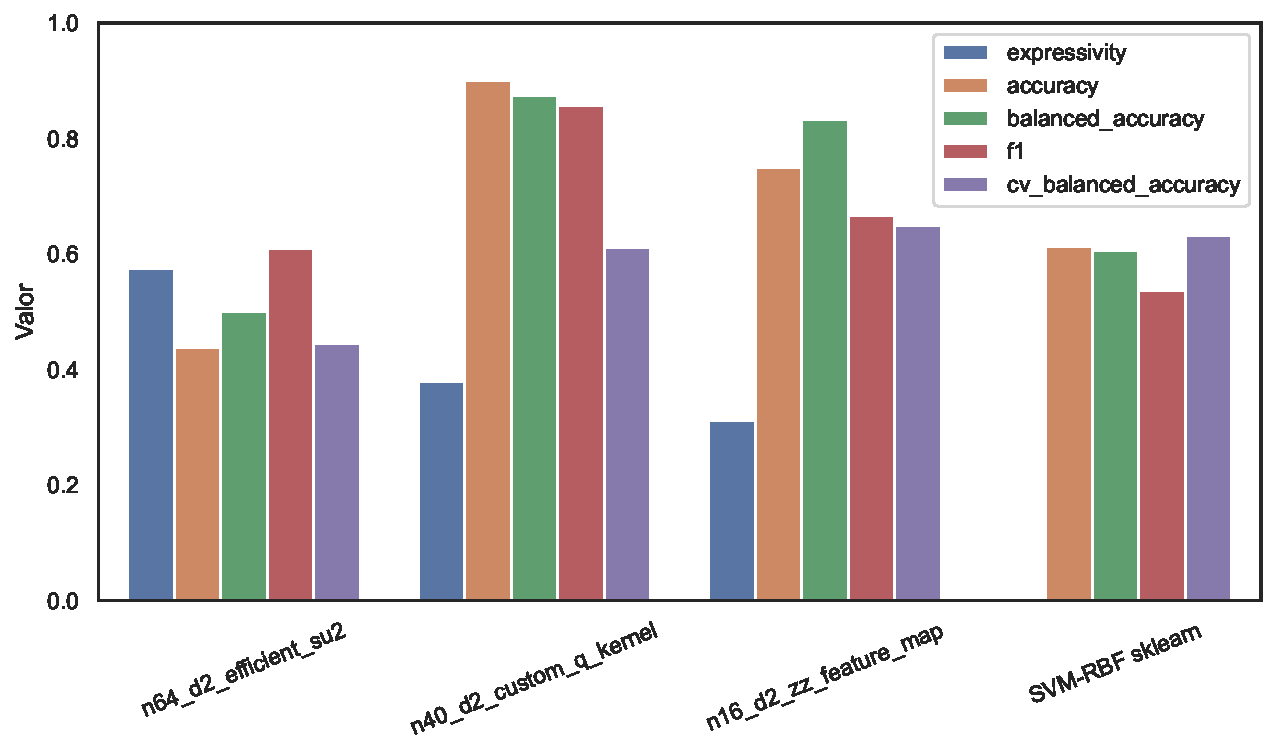
\includegraphics[width=.82\textwidth]{grupo_mayor_expresividad_metricas_vs_sklearn.pdf}
\caption{Comparación generada de expresividad, accuracy, balanced accuracy, $F_1$ y validación cruzada balanceada, incluyendo la referencia clásica.}
\end{figure}

\par\medskip\noindent\textbf{Lectura.} EfficientSU2 es el caso más prometedor desde la representación: combina la expresividad más alta, 0.575, con $F_1=0.609$, superior al promedio clásico de 0.537. Esa combinación sugiere que el mapa captura estructura útil aun con pocas muestras y justifica evaluarlo con conjuntos mayores. La evidencia todavía es preliminar: su balanced accuracy es 0.500 y su CV balanceada $0.445\pm0.051$, de modo que el potencial debe confirmarse con más datos y repeticiones externas.

\clearpage
\section{Mejores resultados por tipo y sus limitaciones}
Para no seleccionar únicamente los mejores resultados globales, la Figura~\ref{fig:best-by-type} conserva el mayor accuracy de cada familia. El mapa propio $(48,4)$ es el caso más destacado y ZZ $(16,2)$ ocupa el segundo lugar. EfficientSU2 no lidera por accuracy, pero sobresale por reunir máxima expresividad y un $F_1$ competitivo; por ello es especialmente prometedor como línea futura.

\begin{figure}[H]
\centering
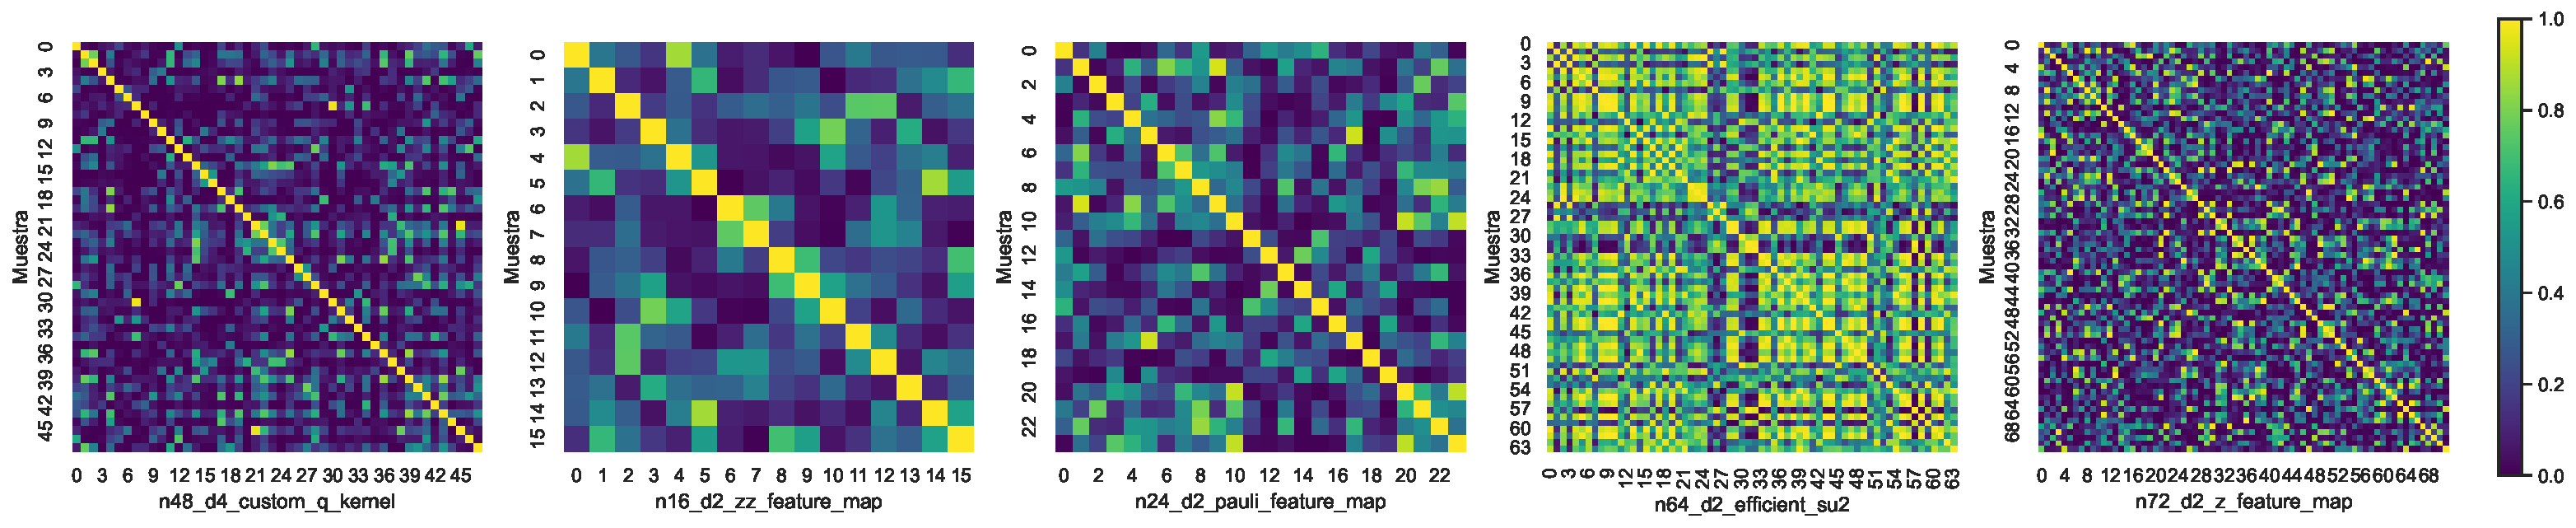
\includegraphics[width=\textwidth]{grupo_mejor_accuracy_por_tipo_heatmaps_escala_0_1.pdf}
\caption{Kernel correspondiente al mayor accuracy observado dentro de cada tipo de mapa.}
\label{fig:best-by-type}
\end{figure}

\begin{table}[H]
\centering\tiny
\caption{Mejor resultado aislado por tipo de mapa.}
\label{tab:best}
\begin{tabular}{rrlccccc}
\toprule
$N$ & $d$ & \textbf{Mapa} & \textbf{Expr.} & \textbf{Acc.} & \textbf{Bal. acc.} & \textbf{$F_1$} & \textbf{CV bal. $\pm$ DE}\\
\midrule
48 & 4 & Propio & 0.161 & 0.917 & 0.900 & 0.889 & $0.555\pm0.098$\\
16 & 2 & ZZ & 0.311 & 0.750 & 0.833 & 0.667 & $0.650\pm0.200$\\
24 & 2 & Pauli Y/ZZ & 0.293 & 0.500 & 0.625 & 0.400 & $0.433\pm0.097$\\
64 & 2 & EfficientSU2 & 0.575 & 0.438 & 0.500 & 0.609 & $0.445\pm0.051$\\
72 & 2 & Z & 0.255 & 0.389 & 0.375 & 0.267 & $0.434\pm0.021$\\
\bottomrule
\end{tabular}
\end{table}

\subsection{Por qué se consideran casos aislados}
El mejor mapa propio obtiene accuracy 0.917 con solo 48 muestras de entrenamiento y una expresividad de 0.161, muy inferior al 0.380 de la configuración propia más expresiva. Además, su accuracy balanceada de test (0.900) contrasta con una CV balanceada de 0.555. Esta brecha, junto con tests de aproximadamente $N/4$ observaciones, hace plausible que el resultado dependa de la partición y de la aleatoriedad.

La misma cautela aplica al resto: las métricas no crecen de forma monótona con la expresividad y cada familia se evaluó en pocas configuraciones. Por tanto, los valores de la Tabla~\ref{tab:best} son \textbf{máximos observados}, no estimaciones robustas del desempeño esperado. Los mapas más expresivos siguen siendo prometedores porque una muestra mayor podría revelar estructura que hoy no se generaliza; esa posibilidad debe validarse con más datos, particiones repetidas y barras de error comparables.

\subsection{Limitaciones experimentales}
\begin{itemize}
  \item Los subconjuntos de entrenamiento varían entre 16 y 72 muestras; una o dos predicciones alteran sustancialmente las métricas.
  \item Solo hay una división externa por configuración. La validación cruzada interna no reemplaza repetir todo el flujo con nuevas semillas.
  \item Cambian simultáneamente $N$, PCA y mapa; no se aísla causalmente el efecto del circuito.
  \item La expresividad usada es el promedio del heatmap, incluida la diagonal; debe complementarse con alineamiento, rango efectivo y separación intra/interclase.
  \item El costo de construir el kernel completo es $O(N^2)$, lo que limita el escalado al dataset completo.
\end{itemize}

\clearpage
\section{Ruido de la máquina: kernel ideal frente a H2}
El repositorio compara EfficientSU2 $(N,d)=(40,3)$ calculado idealmente con las matrices obtenidas en H2. La tercera matriz de cada panel representa el error absoluto elemento a elemento,
\begin{equation}
E_{ij}=\left|K^{H2}_{ij}-K^{\mathrm{ideal}}_{ij}\right|.
\end{equation}
\par\noindent Esta visualización evita cancelaciones de signo y muestra dónde la máquina altera la similitud entre pares.

\begin{figure}[H]
\centering
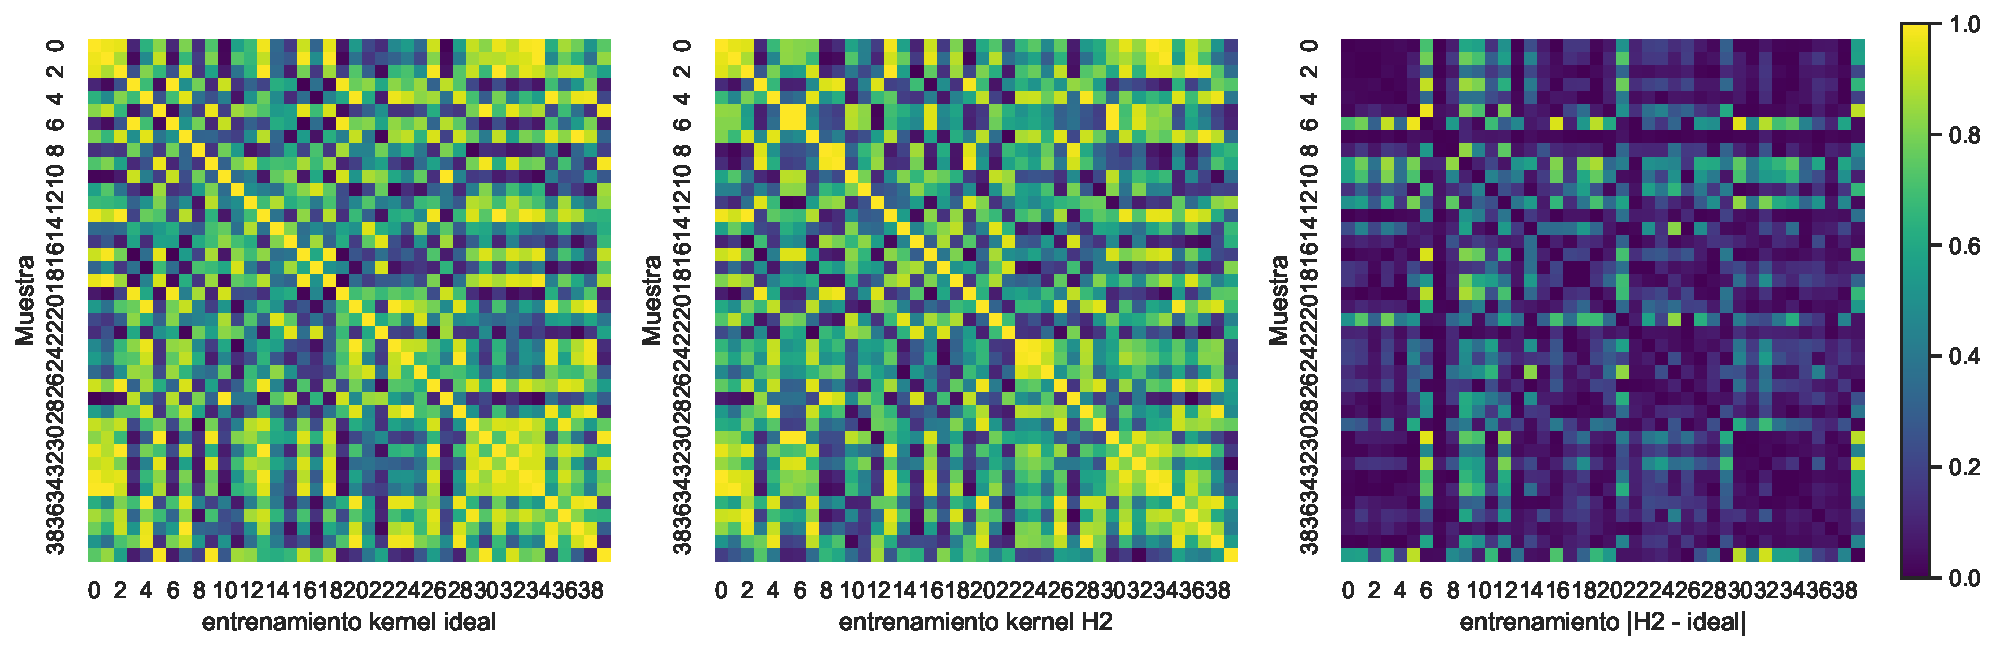
\includegraphics[width=.97\textwidth]{n_40_dim_3_efficient_su2_entrenamiento_kernel_h2_ruido_absoluto.pdf}
\caption{Entrenamiento: kernel ideal, kernel H2 y error absoluto. MAE 0.185 y RMSE 0.287.}
\label{fig:h2-train}
\end{figure}

\begin{figure}[H]
\centering
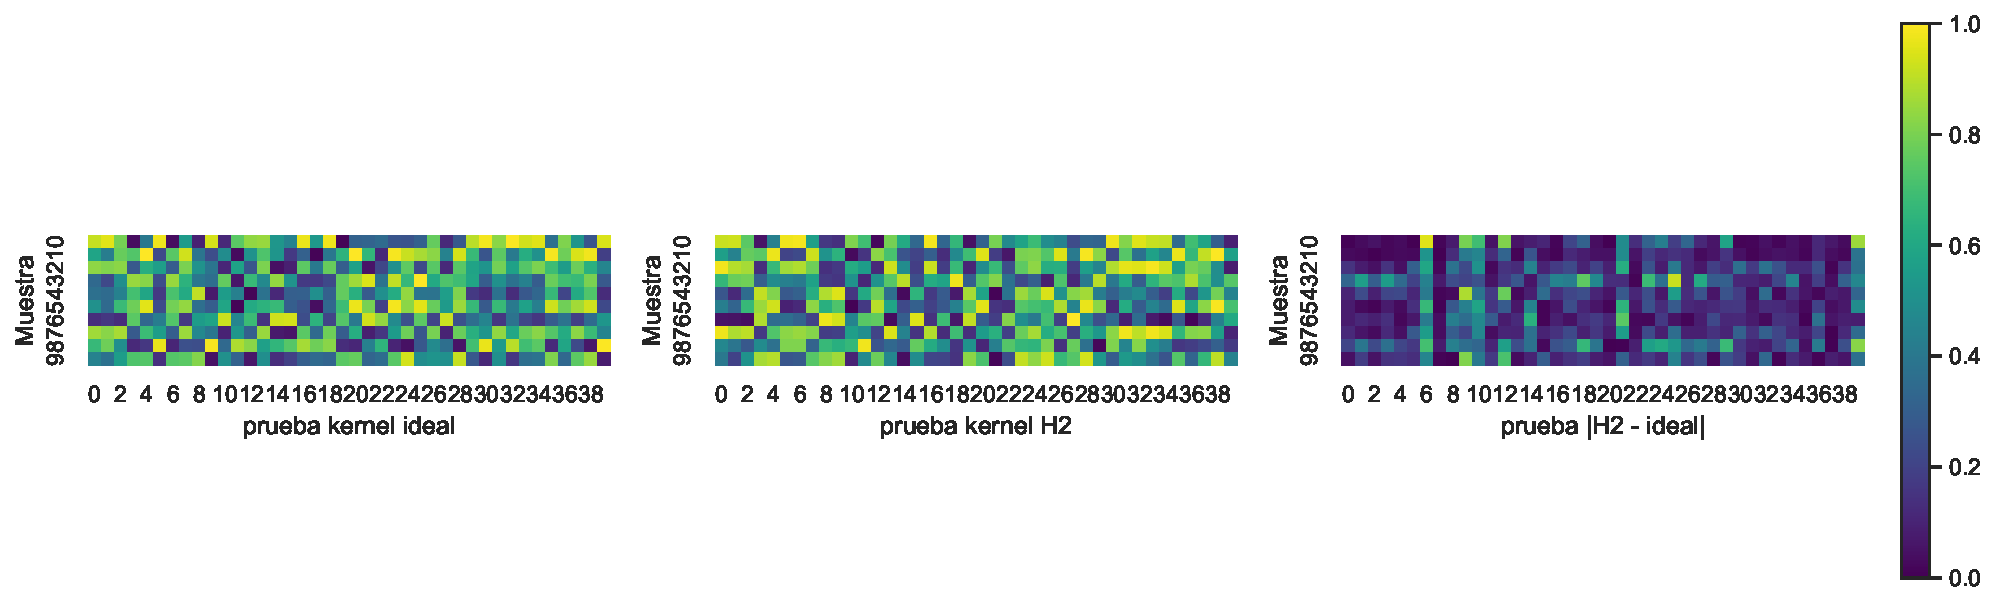
\includegraphics[width=.97\textwidth]{n_40_dim_3_efficient_su2_prueba_kernel_h2_ruido_absoluto.pdf}
\caption{Prueba: kernel ideal, kernel H2 y error absoluto. MAE 0.202 y RMSE 0.282.}
\label{fig:h2-test}
\end{figure}

\par\medskip\noindent
Los errores no son uniformes: aparecen filas, columnas y pares con discrepancias elevadas. El máximo absoluto alcanza 0.974 en entrenamiento y 0.951 en prueba. Esto puede cambiar la geometría entregada a la SVM incluso si la apariencia global de ambos kernels es semejante. Los valores resumen se calcularon directamente de las matrices guardadas en \texttt{data/kernel\_h2/} y \texttt{data/test\_h2/}.

\textbf{Alcance de la comparación.} Este panel mide la diferencia total entre la simulación ideal y H2; no separa error de muestreo, compilación, ruido de compuertas, lectura o deriva. Tampoco basta para afirmar robustez del clasificador. La evaluación final debe repetir ejecuciones de hardware, reportar incertidumbre por elemento y medir cuánto cambia cada métrica de clasificación.

\clearpage
\section{Reproducibilidad, modularidad y escalado}
Las figuras y tablas cuánticas se generan a partir de los datos, matrices y scripts del repositorio. La separación entre preparación, construcción del mapa, generación del kernel, backend y clasificación permite reproducir una configuración o sustituir un componente de forma independiente. La evaluación triangular y la ejecución por lotes reducen trabajo redundante y permiten ampliar gradualmente el número de muestras. Como siguiente paso, deben conservarse los mismos índices para SVM y QSVM, fijarse semillas y repetirse al menos tres particiones externas.

\section{Trabajo futuro: consolidar los mapas prometedores}
El siguiente ciclo experimental debe concentrarse en dos señales complementarias. El \textbf{mapa propio} produjo el mejor resultado aislado, con accuracy 0.917, balanced accuracy 0.900 y $F_1=0.889$; la prioridad es comprobar si ese desempeño persiste al repetir particiones y aumentar la muestra. \textbf{EfficientSU2}, por otra parte, produjo la mayor expresividad (0.575), un $F_1$ competitivo de 0.609, profundidad 10 y ninguna compuerta de dos qubits en la configuración evaluada. Esta combinación de representación rica y circuito ligero es especialmente prometedora para escalar el experimento.

\begin{enumerate}
  \item \textbf{Aumentar datos de forma progresiva.} Evaluar ambos mapas con subconjuntos crecientes, manteniendo índices y balance de clases comunes con la SVM-RBF. La hipótesis principal es que la alta expresividad de EfficientSU2 puede traducirse en mejor generalización cuando exista suficiente diversidad de muestras.
  \item \textbf{Explorar la arquitectura EfficientSU2.} Variar de forma controlada el número de qubits, repeticiones y topología de entrelazamiento. Su configuración actual evita compuertas de dos qubits, lo que reduce exposición al ruido; versiones más amplias deben buscar mayor capacidad sin perder esa ventaja de profundidad.
  \item \textbf{Confirmar estabilidad estadística.} Repetir todo el flujo con varias semillas externas, reportar intervalos de confianza y comparar las distribuciones de accuracy, balanced accuracy y $F_1$, no únicamente el mejor test.
  \item \textbf{Cerrar la brecha ideal-hardware.} Repetir EfficientSU2 en H2 con distintos presupuestos de shots, caracterizar el error absoluto y evaluar mitigación de ruido. La meta es determinar si su expresividad permanece útil después de la ejecución física.
  \item \textbf{Aprovechar el diseño modular.} Reutilizar kernels persistidos, ejecución por lotes y evaluación triangular para ampliar $N$ sin duplicar circuitos. Esto permite estudiar más datos y backends conservando un protocolo reproducible.
\end{enumerate}

\callout{Hipótesis de trabajo: EfficientSU2 es el candidato con mayor potencial de crecimiento por combinar máxima expresividad, $F_1$ competitivo y bajo costo de compuertas de dos qubits; el mapa propio es la referencia de desempeño que debe reproducirse.}

\section{Conclusión}
El método propuesto ofrece una base altamente reproducible, modular y operativamente escalable para comparar kernels ideales y de hardware. El mapa propio produce el mayor resultado aislado, mientras EfficientSU2 combina la expresividad más alta con un $F_1$ competitivo, lo que lo vuelve especialmente prometedor para experimentos futuros con más muestras. La optimización geométrica reduce casi a la mitad las evaluaciones de entrenamiento, aunque el costo asintótico sigue siendo cuadrático. Finalmente, el error absoluto entre el kernel ideal y H2 confirma que cualquier conclusión sobre hardware debe incorporar ruido e incertidumbre de ejecución.

\begin{multicols}{2}
\bibliographystyle{plain}
\bibliography{references}
\end{multicols}

\end{document}
